\chapter{Antécédents}

\section{Test Designer}
La solution Test Designer permet de générer des référentiels de tests fonctionnels à partir de modèles UML pour le test\footnote{Parmi les différentes approches du test logiciel, MBT (Model Based Testing) a pour objectif de créer des cas de test à partir de modèles abstraits, par exemple en UML\footnote{Unified Modelling Language}}. Elle fait le lien entre la modélisation de tests et le management de tests.

%Figure 
\begin{figure}[!ht]
\centering
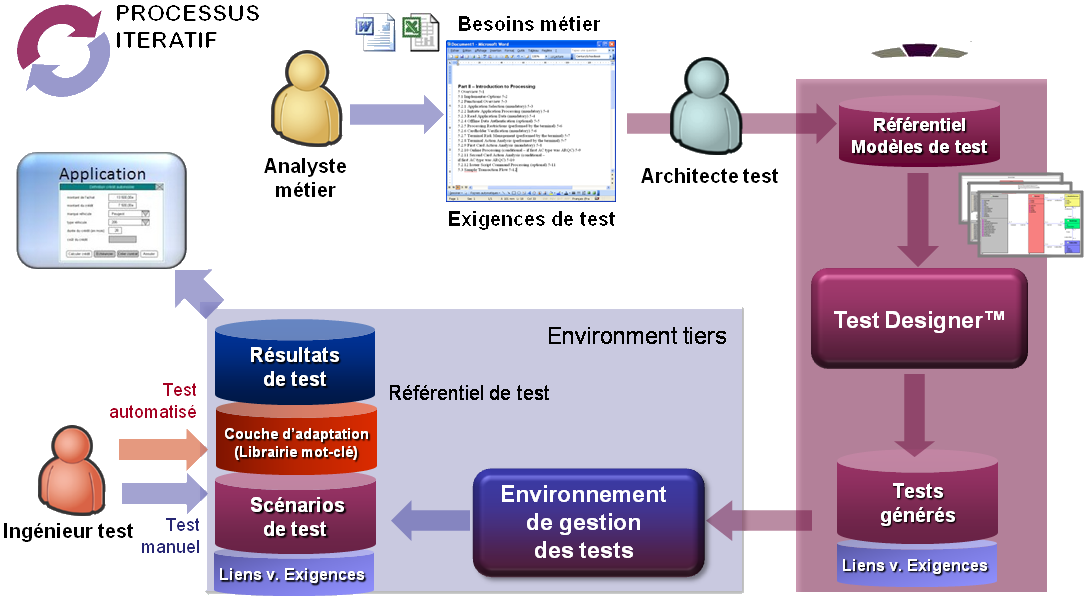
\includegraphics[width=\textwidth]{Illustrations/TheSolutionSmartesting.png}
\caption{La solution Smartesting}
\label{figure:La Solution Smartesting}
\end{figure}

\subparagraph*{}
La modélisation de tests se fait à l'aide de modeleurs UML basés sur Eclipse\footnote{Eclipse est une plateforme applicative sur laquelle peuvent se greffer des applications clientes sous forme de plugins(extensions)}. Les modeleurs supportés actuellement par Test Designer sont Borland Together 2008 et IBM Rational Software Modeler 7.0.5 \& 7.5. Il s'agit de modeleurs basés sur la plateforme Eclipse. Eclipse est une architecture de plugins qui communiquent les uns avec les autres pour former une application. C'est via ce mécanisme que Smartesting a développé deux plugins d'exportation de modèle pour les deux modeleurs précédemment cités.

\subparagraph*{}
Une fois le modèle de tests exporté il est utilisable par Test Designer pour générer automatiquement des référentiels de tests. Ces tests sont stockés dans un référentiel de test. Ces test pourront être publiés vers des environnements tiers (HP Quality Center, tests JUnit, XML, Spécifications pdf...).

\subparagraph*{}
Le processus de génération de tests de la solution Smartesting est un processus itératif. C'est à dire que si l'application déjà testée doit évoluée, la prise en compte des nouvelles fonctionnalités, ne générera pas un nouveau coût de génération des tests. 
Il suffit de modifier le modèle UML de spécifications via le modeleur, puis de générer les tests à nouveau (automatique). Ainsi les architectes de test gagnent un temps considérable à ne pas générer des test qui sont déjà existants.

\subparagraph*{}
Traditionnellement la génération de tests est effectuée manuellement par un ingénieur de tests.

\section{Environnement de travail}
La première tâche qui m'a été confiée à mon arrivée fut d'installer mon poste de travail. Un ordinateur avec Ubuntu 8.10 m'a été confié et j'y ai installé IntelliJ Idea 8.0 (IDE\footnote{Environnement de développement intégré}), adapter quelques options de configuration au développement sur le projet Test Designer. Je me suis ensuite familiarisé pendant une semaine avec le code existant. La consigne était de ne demander d'aide de personne pendant une semaine. Au début de la semaine qui suivit, je devais faire une compte rendu de ce que j'avais compris. Ce ``test'' permet en fait à l'équipe d'avoir un  marqueur sur la lisibilité du code source. Après cette phase d'apprentissage de l'existant, j'ai commencé à travailler sur des fonctionnalités de Test Designer.

\subparagraph*{}
Le code source de Test Designer (le coeur de métier de Smartesting) est développée en JAVA avec un moteur de génération de tests qui s'appuie sur une approche prover (en c++). L'injection de dépendances est gérée par PICO. Une grande variété de bibliothèques sont utilisées telles que les google collections, JUnit, Mockito, JTidy, ou encore JYaml. Certaines ``boîtes à outils'' sont néanmoins développés en interne pour les besoins de la production. Les plugins dans les modeleurs utilisent l'architecture en plugin d'Eclipse pour s'y intégrer. En ce qui concerne les publishers, ils sont un fichier XML créé à partir du référentiel de tests. Ce fichier est ensuite exploité par le biais d'une API développée par l'équipe est distribuée aux clients lors de la livraison. Finalement l'API est aussi bien utilisée par les développeurs de l'équipe R\&D, les consultants de Smartesting que les clients finaux.

\section{Objectifs visés}
Les objectifs qui m'ont été fixés correspondent à ceux de l'équipe. C'est à dire la sortie de la version 3.4 de Test Designer. En effet je suis arrivé peu après la sortie de la version 3.3. Ce fut un avantage pour moi car j'ai pu voir le deroulement d'un jalon dans son intégralité.